\textbf{Исходный текст:} \\
    Hello!

\textbf{Публичный ключ $(e, n)$:} \\
    (1336750571917222506367500878005, 8085472216604733526839569321341)

\textbf{Приватный ключ $(d, n)$:} \\
    (1478409329065133370310312496101, 8085472216604733526839569321341)

\textbf{Зашифрованный текст:} \\
    5807241446759901267216605390094 1945721761216314545617066200940
    1389314913534850043257468141227 1389314913534850043257468141227
    6572208100939281410200927429783 3016927945680088341886714157792
    ~~~~~~~~~~~~~~~~~~~~~~~~~~~~~~~

Результаты работы программы представлены на рисунках~\ref{ris:encode-test-1}-\ref{ris:decode-test-1}.

\vspace{\baselineskip}
\begin{figure}[H]
\center{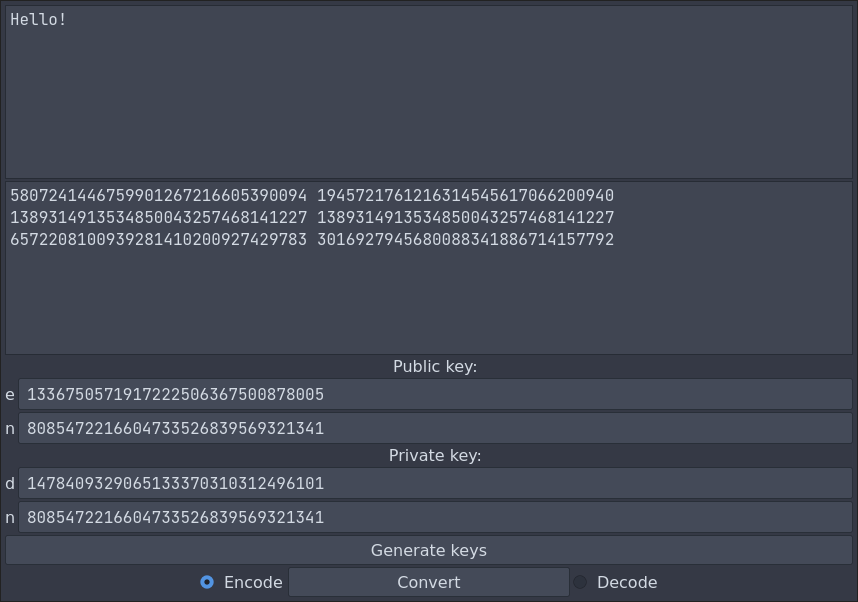
\includegraphics[width=0.8\linewidth]{figures/encode-test-1}}
    \caption{Шифрование}
\label{ris:encode-test-1}
\end{figure}

\vspace{\baselineskip}
\begin{figure}[H]
\center{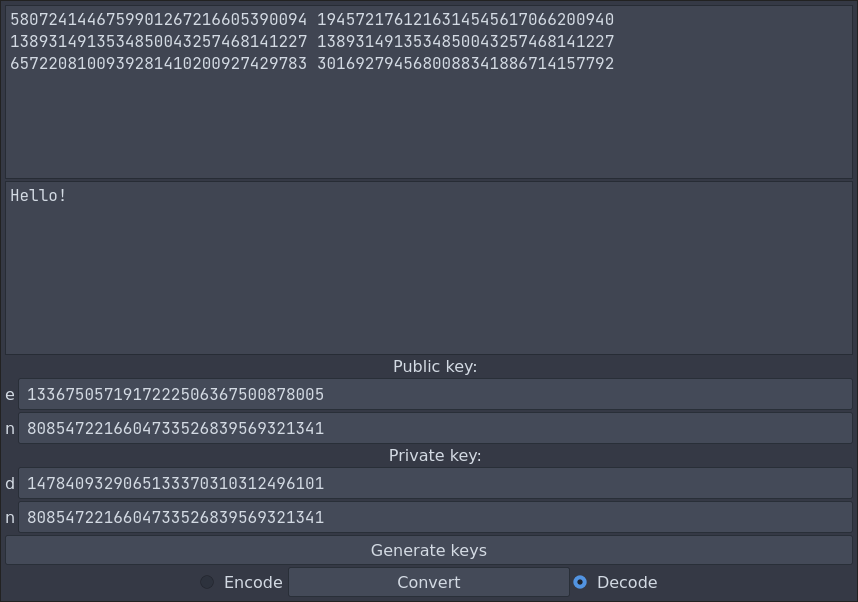
\includegraphics[width=0.8\linewidth]{figures/decode-test-1}}
    \caption{Расшифрование}
\label{ris:decode-test-1}
\end{figure}
